\section{Model assessment}

Given a dataset $\mathcal{D}=\left\{ \textbf{x}_i,t_i \right\}$ with $i=1,\ldots, N$, we can choose a model based on the computed loss $L$ on $\mathcal{D}$.
For regression, the loss function is defined as:
\[L_{train}=\dfrac{1}{N}\sum_{n=1}^N{\left(t_n-y(\textbf{x}_n)\right)}^2\]
And for classification, the loss function becomes:
\[L_{train}=\dfrac{1}{N}\sum_{n=1}^N I(t_n \neq y(\textbf{x}_n))\]
The training error decreases as the model complexity increases.

However, it's important to note that the training error doesn't give an accurate estimate of the error on new data, known as the prediction error.
For regression, the prediction error is represented as:
\[L_{true}=\iint{\left( t-y(\textbf{x})\right)}^2\text{P}(\textbf{x},t)d\textbf{x}dt \]
And for classification, it is:
\[L_{true}=\iint I(t\neq y(\textbf{x}))\text{P}(\textbf{x},t)d\textbf{x}dt \]
Unfortunately, modeling the joint probability distribution $\text{P}(\textbf{x},t)$ is often not feasible.
\begin{figure}[H]
    \centering
    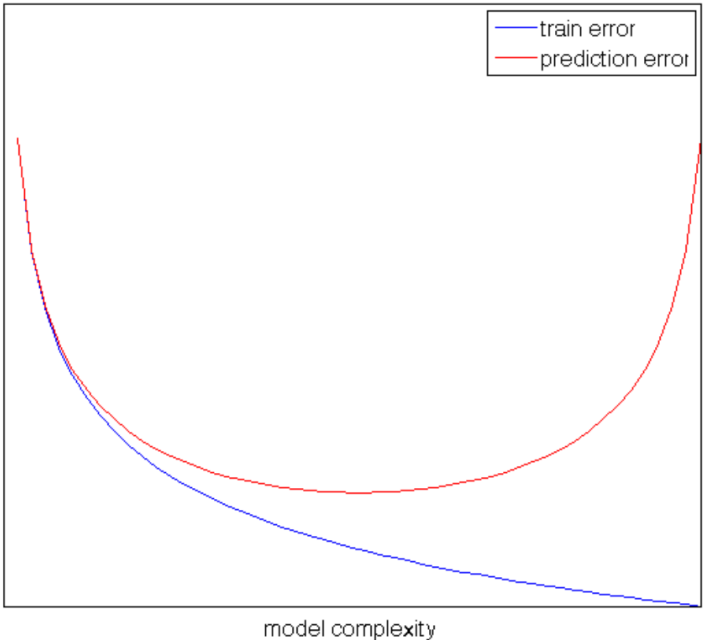
\includegraphics[width=0.35\linewidth]{images/error.png}
    \caption{Train error compared to prediction error}
\end{figure}

\paragraph*{Practical application}
In practical scenarios, data is typically randomly split into a training set and a test set. 
Model parameters are optimized using the training set, and the prediction error is estimated using the test set. 
For regression, this estimation yields:
\[L_{test}=\dfrac{1}{N_{test}}\sum_{n=1}^{N_{test}}{\left(t_n-y(\textbf{x}_n)\right)}^2\]
And for classification:
\[L_{test}=\dfrac{1}{N_{test}}\sum_{n=1}^{N_{test}}I(t_n\neq y(\textbf{x}_n))\]
\begin{figure}[H]
    \centering
    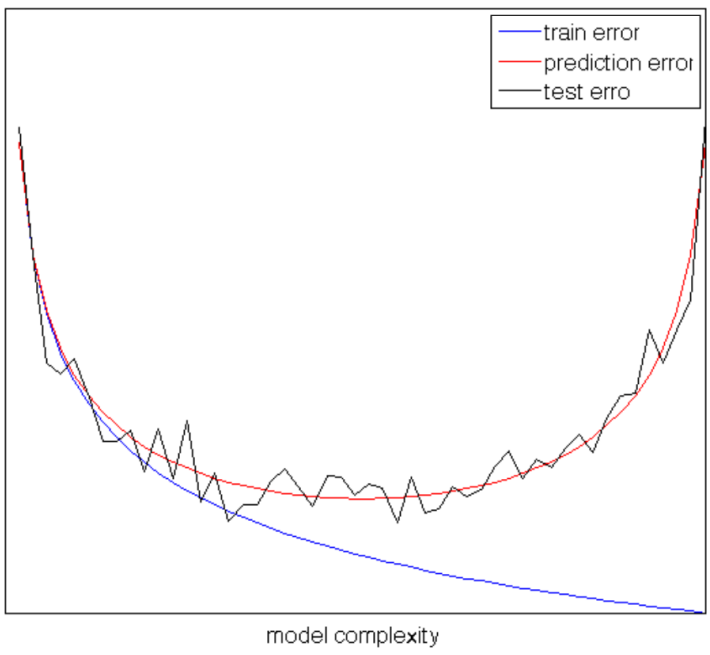
\includegraphics[width=0.35\linewidth]{images/error1.png}
    \caption{Error in practice}
\end{figure}
As the number of data points increases, these errors tend to converge, as depicted in the following figure:
\begin{figure}[H]
    \centering
    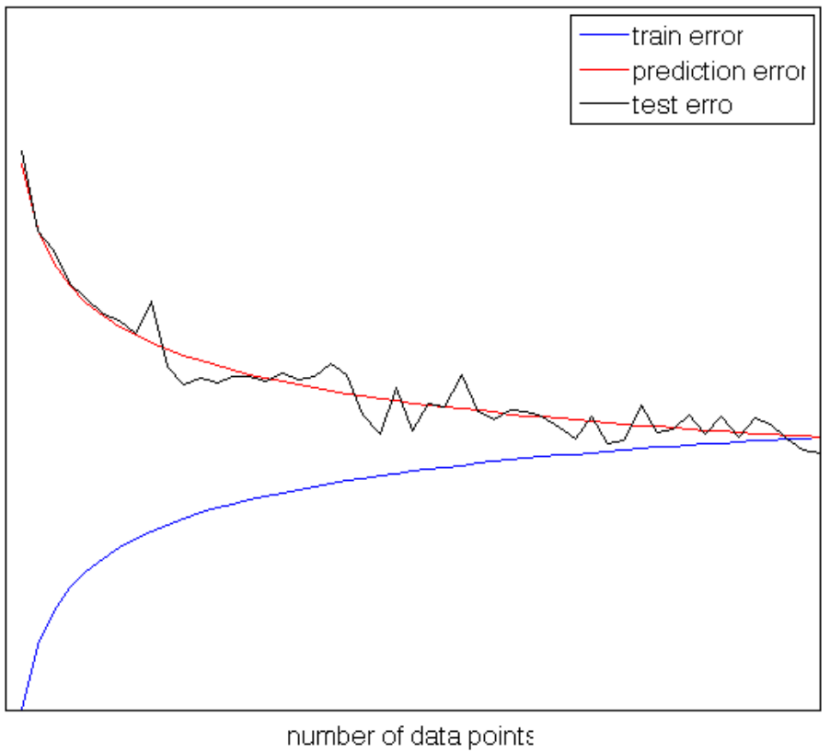
\includegraphics[width=0.35\linewidth]{images/error2.png}
    \caption{Error in function of the number of data points}
\end{figure}
Analyzing the train-test errors helps identify potential issues:
\begin{itemize}
    \item \textit{High bias}: when both training and test errors are higher than expected and close to each other.
    \item \textit{High variance}: when the training error is significantly lower than expected and gradually approaches the test error.
\end{itemize}

\paragraph*{Problems}
Frequently, data availability is constrained, and the test error tends to be minimal, leading to potential overestimation or underestimation of prediction error.
Utilizing test error for model selection can result in overfitting to the test set.
An unbiased estimate of prediction error is achievable only if the test set remains separate from both training and model selection phases.

\subsection{Optimal model}
To select the optimal model and determine the appropriate hyperparameters, we initially partition the data into three subsets: training data, validation data, and test data. 
The process involves the following steps:
\begin{enumerate}
    \item Utilize the training data to train the model parameters.
    \item For each trained model, assess its performance using the validation data to compute the validation error.
    \item Identify the model with the lowest validation error, and subsequently, employ the test data to estimate the prediction error.
\end{enumerate}
However, for this approach to be dependable, it's imperative that the validation data set is sufficiently sizable, especially in comparison to the training data set. 
Otherwise, there's a risk of overfitting to the validation data, potentially leading to the selection of a suboptimal model.

\paragraph*{Leave-one-out cross validation}
Leave-one-out cross-validation (LOO-CV) involves training the model on all samples in the dataset $\mathcal{D}$ except for a single sample $\{\textbf{x}_i,t_i\}$, and then evaluating the model's performance on that omitted sample. 
The prediction error estimate of our model is then computed as the average error across all single-sample evaluations:
\[L_{LOO}=\dfrac{1}{N}\sum_{i=1}^{N}{\left( t_i-y_{\mathcal{D}_i}(\textbf{x}_i) \right)}^2\]
Here, $y_{\mathcal{D}_i}$ represents the model trained on $\mathcal{D}$ excluding $\{\textbf{x}_i,t_i\}$. 

The $L_{\text{LOO}}$ estimate of prediction error provides an almost unbiased assessment (slightly pessimistic). 
However, LOO-CV is computationally intensive due to its requirement to repeatedly train models on nearly all data points.

\paragraph*{K-fold cross validation}
K-fold cross-validation involves randomly dividing the training data $\mathcal{D}$ into $k$ folds: $\mathcal{D}_1,\mathcal{D}_2,\dots,\mathcal{D}_k$. 
For each fold $\mathcal{D}_i$, the model is trained on $\mathcal{D}$ excluding $\mathcal{D}_i$, and then the error is computed on $\mathcal{D}_i$ as follows:
\[L_{\mathcal{D}_i}=\dfrac{k}{N}\sum_{(\textbf{x}_n,t_n) \in \mathcal{D}_i} {\left( t_n-y_{\mathcal{D}\setminus\{\mathcal{D}_i\}}(\textbf{x}_n) \right)}^2\]
Finally, the prediction error is estimated as the average error computed across all folds:
\[L_{k-fold}=\dfrac{1}{k}\sum_{i=1}^{k}L_{\mathcal{D}_i}\]

The $L_{k\text{-fold}}$ estimate of prediction error provides a slightly biased (pessimistic) assessment but is computationally less expensive. 
Typically, $k$ is set to ten.

\paragraph*{Other metrics}
Various metrics are employed to evaluate models by adjusting their training error based on their complexity:
\begin{itemize}
    \item Mallows's $C_p$: 
        \[C_p=\dfrac{1}{N}\left( \text{RSS}+2M\sigma^2 \right)\]
    \item Akaike Information Criteria:
        \[\text{AIC}=-2\ln(L)+2M\]
    \item Bayesian Information Criteria: 
        \[\text{BIC}=-2\ln(L)+M\ln(N)\]
    \item Adjusted $R^2$:
        \[A_{R^2}=1-\dfrac{\text{RSS}/(n-m-1)}{\text{TSS}/(N-1)}\]
\end{itemize}
Here, $M$ represents the number of parameters, $N$ denotes the number of samples, $L$ signifies the loss function, $\sigma^2$ stands for the estimate of noise variance, RSS corresponds to the residual sum of squares, and TSS indicates the total sum of squares.

AIC and BIC are typically utilized when maximizing the log-likelihood. 
BIC tends to penalize model complexity more severely compared to AIC.\@